\subsubsection{Ethereum Virtual Machine}
\label{sec:evm}
The Ethereum Virtual Machine (\textbf{EVM}) is an abstract computing machine
that enables the nodes of the Ethereum network to execute smart-contract
codes.


\autoref{fig:evm} shows the components of the Ethereum Virtual Machine.
The dashed lines represents the fact that there exists an EVM instruction
that allows the transfer of data from one component to another.
\begin{figure}
	\begin{center}
		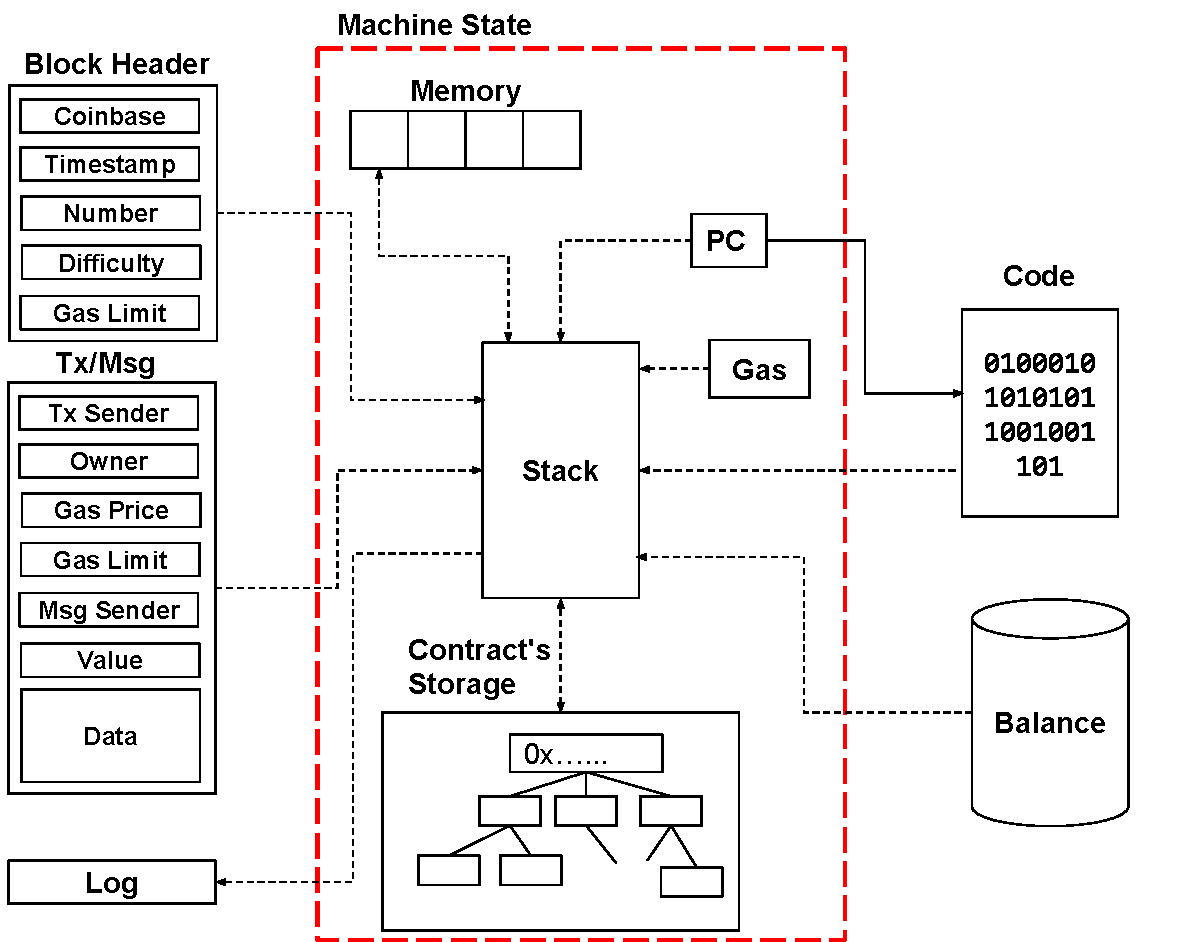
\includegraphics[width=0.7\textwidth]
        {./res/img/evm-overview.pdf}
	\end{center}
	\caption{Overview of the Ethereum Virtual Machine}
	\label{fig:evm}
\end{figure}
Like the JVM, the EVM is a stack-based machine. In this system the word size
and the stack item size are both $256$--bit\footnote{The motivation
for this choice is to facilitate the Keccak-256 hash scheme and elliptic
curve computation that are pervasive in Ethereum.},
and the stack capacity is $1024$.
The EVM memory consists of a simple byte array and exists only during the
execution. The size of this array is allocated using an on-demand logic.
The storage is a key value hash table (stored as a merkle tree) that is
persistent and is part of the state of the contract account.
The program is stored on the blockchain and therefore cannot
be modified\footnote{There exist
techniques based on the strategy pattern to provide new smart-contract version
updates as explained here:
\url{https://ethereum.stackexchange.com/questions/2404/upgradeable-smart-contracts}}.
In addition to the aforementioned structures the EVM can read the information
provided in the transaction/message that initiated the execution. In particular
the EVM can access the input field, which contains the arguments for a peculiar
execution.
For a full instruction list and specification of the EVM
we refer to the official specification~\cite[Appendix H]{wood2018ethereum}.


Unlike the Bitcoin's \textit{Script} language~\cite{bib:masteringbitcoin} the
Ethereum Virtual Machine can express and supports the execution of loops.
To avoid the abuse of the resources (CPU and storage) of the full nodes
forming the network, Ethereum introduces the concept of
\textbf{gas}~\cite{wood2018ethereum}, which was described
in~\autoref{sec:tx-execution}. In this
execution model each instruction and increase in the size of the memory or
storage are bound to a cost expressed in gas.

%~ The price of a gas unit
%~ is known as \textbf{gas price} and is bound to a particular execution.
%~ Indeed this price is specified in the transaction or in the message call
%~ which originates the execution. The higher this price the higher the
%~ possibility that the  transaction will be included in the blockchain.
%~ Usually the miners advertise the minimum gas price they are willing to accept.
%~ Another important concept specified in the transaction is the
%~ \textbf{gas limit}, i.e. the maximum gas amount the executor is willing to
%~ consume for this particular execution.

Before executing a \emph{smart contract}, i.e. a program on the EVM, the
initiator of the transaction allocates a certain amount of gas that it is
willing to spend for this execution.
If during the execution all the gas is consumed an \textbf{Out of gas exception}
is raised.


%~ Thanks to this brief introduction we can already understand some crucial
%~ mechanisms involved in Ethereum and their motivation:
%~ \begin{itemize}
	%~ \item A transaction is not valid if the originator of a transaction have
	%~ a balance lower than \verb|gas_price * gas_limit| \verb|+|
	%~ \verb|transaction_value|:
	%~ it means that it cannot afford the execution. In fact this value is
	%~ deducted upfront and later the remaining gas are refund.
	%~ \item If during the execution the gas limit is exceeded an Exception
	%~ (\textbf{Out of gas exception}) is raised, and the funds are not returned,
	%~ because the execution already took place.
%~ \end{itemize}


The \textbf{machine state} represents the current configuration of the Ethereum
Virtual Machine interpreter. It consists of the remaining gas, the program
counter, the memory and the stack.

As already explained in~\autoref{sec:tx-execution}, a transaction can trigger
the execution of contract creations and message calls. In turn, these can invoke
the execution of other contract creations and other message calls. To deal with
this eventuality, the EVM has at its disposal a \textbf{call stack}: when a new
contract call or message call is executed, the current machine state is stored
on the call stack and a new machine state with the invoked code is created. When
the invoked code terminates, its activation record is popped from the call stack
and a return status flag is put on the activation record of the invoker: $1$
indicates that the code threw an exception and $0$ indicates a successful
termination. The call stack's depth is limited to
$1024$~\cite{wood2018ethereum}. Although the yellow paper does not define
explicitly the call stack, more details can be found in the
literature~\cite{grishchenko2018semantic} and in the go ethereum
implementation\footnote{An example of use of the call stack is the function
\texttt{opCallCode} in the file \path{core/vm/instructions.go}: it is clear that
the implementation exploits the usual function call stack of the language to
implement the EVM call stack.}.
